\documentclass[rmp,10pt,onecolumn,fleqn,notitlepage]{revtex4-1}

\usepackage{graphicx}
\usepackage{color}
\usepackage{latexsym,amsmath}
\usepackage{physics}
\usepackage{tabularx}
\usepackage{float}
\usepackage{siunitx}
\usepackage{amssymb}
\usepackage{bbold} % to represent identity
\usepackage[caption=false]{subfig} % sfancula la formattazione delle figure se caption è messo su true

% Listing packages
\usepackage{xcolor}
\usepackage{listings}
\usepackage{framed}
\usepackage{inconsolata} % To change the listing font

% URL package and setting
\definecolor{linkcolor}{rgb}{0.65,0.16,0.16}%hyperlink
\usepackage[pdftex,colorlinks=true, pdfstartview=FitV, linkcolor= linkcolor, citecolor= linkcolor, urlcolor= linkcolor, hyperindex=true,hyperfigures=true]{hyperref} %hyperlink%

\usepackage{fancyhdr} % To change page setting

% PAGE SETTING
\pagestyle{fancyplain}
\fancyhf{}
\fancyfoot[R]{\thepage}
\fancyfoot[L]{\today}
\fancyhead[L]{\textbf{Week 9 Report, Quantum Information and Computing (2020)}}
\fancyhead[R]{\textbf{Alice Pagano}}
\renewcommand{\headrulewidth}{0.1pt}
\renewcommand{\footrulewidth}{0.1pt}

% LISTING SETTINGS
\definecolor{cadmiumred}{rgb}{0.89, 0.0, 0.13}
\definecolor{codegray}{rgb}{0.5,0.5,0.5}
\definecolor{commentcolour}{rgb}{0.43,0.63,0.65}
\definecolor{darkgreen}{rgb}{0.0, 0.5, 0.0}

\lstdefinestyle{Fortran}{language=Fortran,
    backgroundcolor=\color{white},
    commentstyle=\color{commentcolour},
    keywordstyle=\bfseries\color{cadmiumred},
    numberstyle=\tiny\color{codegray},
    stringstyle=\color{darkgreen},
    basicstyle=\ttfamily\footnotesize,
    breakatwhitespace=false,
    breaklines=true,
    captionpos=b,
    keepspaces=true,
    numbers=left,
    numbersep=5pt,
    showspaces=false,
    showstringspaces=false,
    showtabs=false,
    tabsize=2,
    frame=single,
    framexleftmargin=11pt,
    %rulecolor=\color{cadmiumred}
}
%\lstset{style=Fortran}

\lstdefinestyle{Gnuplot}{
    backgroundcolor=\color{white},
    commentstyle=\color{commentcolour},
    basicstyle=\ttfamily\footnotesize,
    breakatwhitespace=false,
    breaklines=true,
    captionpos=b,
    keepspaces=true,
    showspaces=false,
    showstringspaces=false,
    showtabs=false,
    tabsize=2,
    frame=single,
    framexleftmargin=11pt,
    rulecolor=\color{cadmiumred}
}

\lstdefinestyle{Python}{language=Python,
    backgroundcolor=\color{white},
    commentstyle=\color{commentcolour},
    keywordstyle=\color{darkgreen},
    numberstyle=\tiny\color{codegray},
    stringstyle=\color{cadmiumred},
    basicstyle=\ttfamily\footnotesize,
    breakatwhitespace=false,
    breaklines=true,
    captionpos=b,
    keepspaces=true,
    numbers=left,
    numbersep=5pt,
    showspaces=false,
    showstringspaces=false,
    showtabs=false,
    tabsize=2,
    frame=single,
    framexleftmargin=11pt
}

% BIBLIOGRAPHY FILE AND SETTING
\begin{filecontents*}{\jobname.bib}
    @article{cite1,
      title={Error handling in Fortran 2003},
      author={Koen Poppe and Ronald Cools and Bart Vandewoestyne},
      journal={ACM Sigplan Fortran Forum},
      year={2012},
      volume={31},
      pages={7-19}
    }
\end{filecontents*}

\bibliographystyle{aipnum4-1}
\setcitestyle{numbers,square}


% Highilight formulas
\newcommand{\mathcolorbox}[2]{\colorbox{#1}{$\displaystyle #2$}}
\newcommand{\hlfancy}[2]{\sethlcolor{#1}\hl{#2}}





\begin{document}



\title{Week 9: Quantum Ising Model}
\author{Alice Pagano}
\date{\today}

\begin{abstract}
In this Report, we initilize and diagonalize the Hamiltonian of an Ising model with \( N \) spin-$1/2$ particles in a one-dimensional lattice. In particular, we study the energy spectrum as a function of the interaction strength \(
\lambda  \).
\end{abstract}

\maketitle


\section{Theory}
The \textbf{quantum Ising model} represents one of the simplest nontrivial many-body quantum system. Let us consider a linear chain of $N$ interacting spins $1/2$ in presence of an external field of \emph{intensity} $\lambda$. The Hamiltonian of the model reads:
\begin{equation}
  H = \sum_{i=1}^{N-1} H_{i,i+1} = \lambda \sum_{i=1}^{N} \sigma _i^{z} + \sum_{i=1}^{N-1} \sigma _{i}^{x} \sigma _{i+1}^{x}
  \label{eq:hamiltonian}
\end{equation}
where \( \sigma  \)s are the Pauli matrices and the coefficient $\lambda$ determines the relative strength of the external field compared to the nearest neighbour interaction.

More particularly, this system features a lattice with nearest neighbour interactions determined by the alignment or anti-alignment of spin projections along the $x$-axis, as well as an external magnetic field perpendicular to the $x$-axis (without loss of generality, along the $z$-axis) which creates an energetic bias for one $z$-axis spin direction over the other.
An important feature of this setup is that, in a quantum sense, the spin projection along the $z$-axis and the spin projection along the $x$-axis are not commuting observable quantities.

% The model can be exactly solved for all coupling constants. In particular:
% \begin{itemize}
% \item when \( \abs{g} < 1 \), the system is said to be in the \textbf{ordered phase}. In this phase the ground state breaks the spin-flip symmetry. Thus, the ground state is in fact \emph{two-fold degenerate}.
%
% \item  when \( \abs{g} < 1 \), the system is said to be in the \textbf{disordered phase}. The ground state preserves the spin-flip symmetry, and is nondegenerate.
%
% \item When \( \abs{g}=1  \), the system undergoes a quantum phase transition.
%
% \end{itemize}

To solve with a numerical simulation the Ising model for \( N \) particles, let us remind that the Pauli matrices can be rewritten in an explicit form as:
\begin{subequations}
\begin{align}
 \sigma _i^z  &= \mathbb{1}_1 \otimes \mathbb{1}_2 \otimes \dots \otimes \sigma _i^z \otimes \dots \otimes \mathbb{1}_N \label{eq:rel_sigma_z}\\
 \sigma _{i}^{x} \sigma _{i+1}^{x} &= \mathbb{1}_1 \otimes \mathbb{1}_2 \otimes \dots \otimes \sigma _i^x \otimes \sigma _{i+1}^x \otimes \dots \otimes \mathbb{1}_N\label{eq:rel_sigma_x}
\end{align}
\end{subequations}


\section{Code Development}

In order to write the hamiltonian of the Ising model for a system with $N$ particles, we develop a program inside the file “ising$\_$hamilt.f90”.

First of all, a user-defined \texttt{FUNCTION} {\bfseries\texttt{tensor$\_$product}}\texttt{(Mat1,Mat2)} is coded for performing the tensor product between two matrices (i.e. between operators) \texttt{Mat1} and \texttt{Mat2}.

\begin{minipage}[t]{0.9\linewidth}%\vspace{0pt}
\begin{lstlisting}[style=Fortran]
! Compute tensor product between two generic matrices
function tensor_product(Mat1,Mat2) result(Tens)
    ...
    N1 = shape(Mat1)
    N2 = shape(Mat2)
    N(1) = N1(1)*N2(1)
    N(2) = N1(2)*N2(2)

    allocate(Tens(N(1),N(2)))

    do ii=1,N1(1),1
        do jj=1,N1(2),1
            do kk=1,N2(1),1
                do mm=1,N2(2),1
                    Tens( (ii-1)*N2(1)+kk, (jj-1)*N2(2)+mm ) = Mat1(ii,jj)*Mat2(kk,mm)
                end do
            end do
        end do
    end do

end function tensor_product\end{lstlisting}
\end{minipage}


Then, the main steps of the program are in order:

\begin{enumerate}

\item the total number of subsystems \texttt{N} and the strength \( \lambda  \) are given as input;

\item the matrix \( \sigma _x \) and \( \sigma _z \) are defined;

\item the total hamiltonian \texttt{H} is computed as the sum between a non-interacting term \texttt{H$\_$non$\_$int} and an interacting one \texttt{H$\_$int} as:

\begin{minipage}[t]{0.65\linewidth}%\vspace{0pt}
\begin{lstlisting}[style=Fortran]
H = lambda*H_non_int(N_part,sigmaz) + H_int(N_part,sigmax)\end{lstlisting}
\end{minipage}

In particular, the two terms are computed by calling:
\begin{itemize}

\item the \texttt{FUNCTION} {\bfseries\texttt{H$\_$non$\_$int}}\texttt{(N,sigmaz)}, which takes in input the number of particles and \( \sigma _z \). It performs the tensor product between \( \sigma _z \) and the identity matrix by exploiting the relationship given by Eq. \eqref{eq:rel_sigma_z}.

\begin{minipage}[t]{0.98\linewidth}%\vspace{0pt}
\begin{lstlisting}[style=Fortran]
! Compute non-interacting term of Ising Hamiltonian
function H_non_int(N, sigmaz) result(H0)

    integer :: N, dim
    integer :: ii, jj, kk
    complex(8), dimension(:,:) :: sigmaz
    complex(8), dimension(:,:), allocatable :: H0
    complex(8), dimension(:,:), allocatable :: tmpMat

    dim = size(sigmaz,1)**N
    allocate(H0(dim,dim))
    allocate(tmpMat(dim,dim))

    H0 = cmplx(0.0,0.0)

    do ii=1,N,1
        tmpMat = tensor_product ( tensor_product( identity(ii-1), sigmaz) , identity(N-ii) )
        H0 = H0 + tmpMat
    end do

end function H_non_int\end{lstlisting}
\end{minipage}

\item the \texttt{FUNCTION} {\bfseries\texttt{H$\_$int}}\texttt{(N,sigmax)}, which takes in input the number of particles and \( \sigma _x \). It performs the tensor product between \( \sigma _x \) and the identity matrix by exploiting the relationship given by Eq. \eqref{eq:rel_sigma_x}.

\begin{minipage}[t]{0.98\linewidth}%\vspace{0pt}
\begin{lstlisting}[style=Fortran]
! Compute interacting term of Ising Hamiltonian
function H_int(N,sigmax) result(H1)

    integer :: N, dim
    integer :: ii, jj, kk
    complex(8), dimension(:,:) :: sigmax
    complex(8), dimension(:,:), allocatable :: H1
    complex(8), dimension(:,:), allocatable :: tmpMat

    dim = size(sigmax,1)**N
    allocate(H1(dim,dim))
    allocate(tmpMat(dim,dim))

    H1 = cmplx(0.0,0.0)

    do ii=1,N-1,1
        tmpMat = tensor_product( tensor_product ( tensor_product( identity(ii-1), sigmax),
                                sigmax ), identity(N-ii-1) )
        H1 = H1 + tmpMat
    end do

end function H_int\end{lstlisting}
\end{minipage}


\end{itemize}


\item then, the Ising hamiltonian is diagonalized by calling the Lapack's routine {\bfseries\texttt{zheev}};

\item the first \texttt{klevels} eigenvalues are stored in order to study the energy spectrum for a fixed number of particles \texttt{N} and strength \texttt{lambda}.


\end{enumerate}

Finally, with a python script “script.py", we execute the program for different \texttt{N} and different \texttt{lambda}. At the end, the first \texttt{klevels} of the energy spectrum for different particles are plotted as a function of \texttt{lambda}.



\section{Results}

We execute the program for $N\in[3:10]$ and \( \lambda \in[0:3] \).
In Fig. \ref{fig:results} the first seven eigenstates as a function of $\lambda$ for different $N$ are shown.

Let us focus on the ground state $E_0$ and on the first excited state of the hamiltonian $E_1$. We can note that for a nill interaction strength they are degenerate, independently on the number of particles used in the simulation.
However, for \( \lambda \neq 0 \), the ground state and the first excited state start to differ. It is interesting to notice that the difference $E_1-E_0$ decrease with higher $N$. This trend is more visible in Fig. \ref{fig:diff}, where the diffeence between the two eigenstates is plotted as a function of \( \lambda  \). It seems that the difference for \( N \rightarrow \infty  \) approaches a zero value for \( \lambda < 1 \), denoting the presence of a quantum phase transition at \( \lambda =1 \).


\begin{figure}[H]
\begin{minipage}[c]{0.49\linewidth}
\subfloat[][4 particles]{ 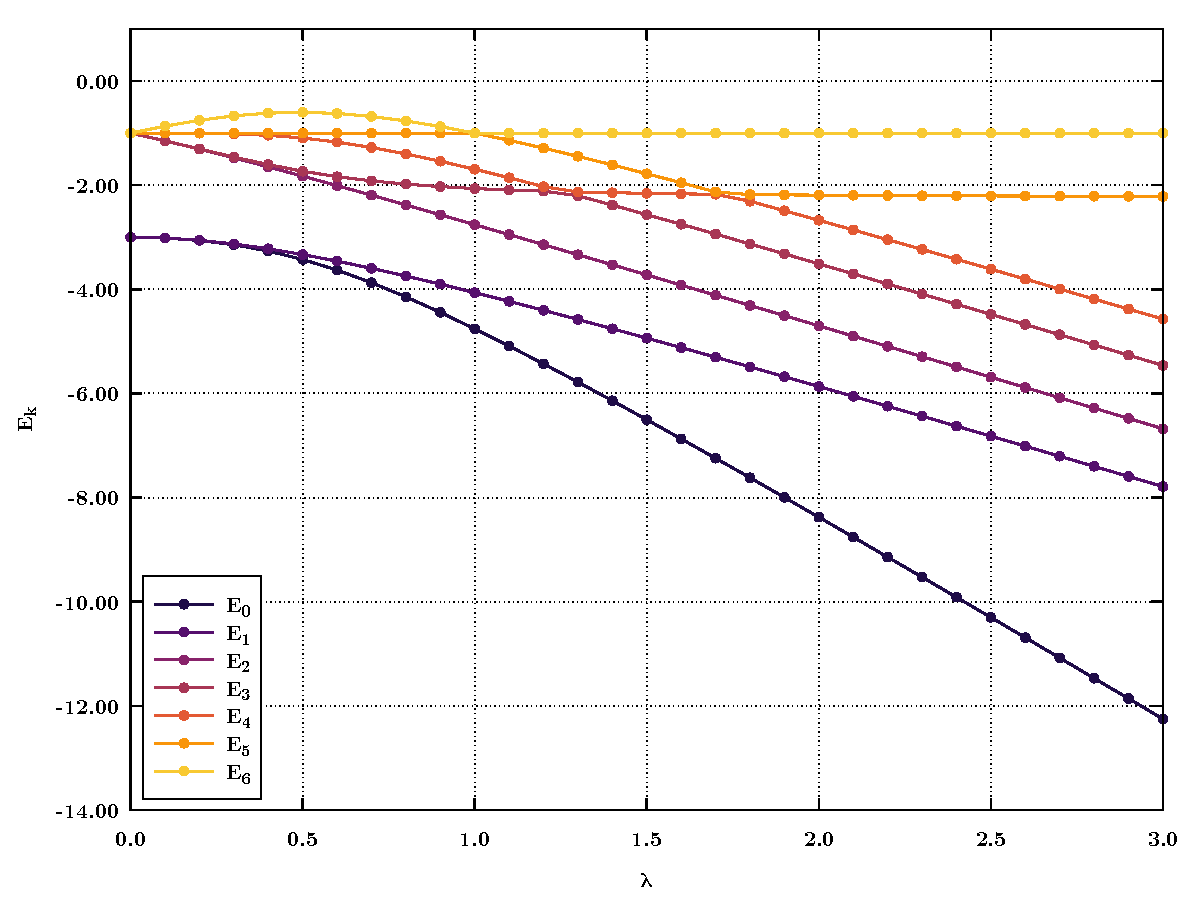
\includegraphics[width=\textwidth]{image/eig_4.pdf} \label{fig:result_(a)} }
\end{minipage}
\begin{minipage}[]{0.49\linewidth}
\centering
\subfloat[][6 particles]{    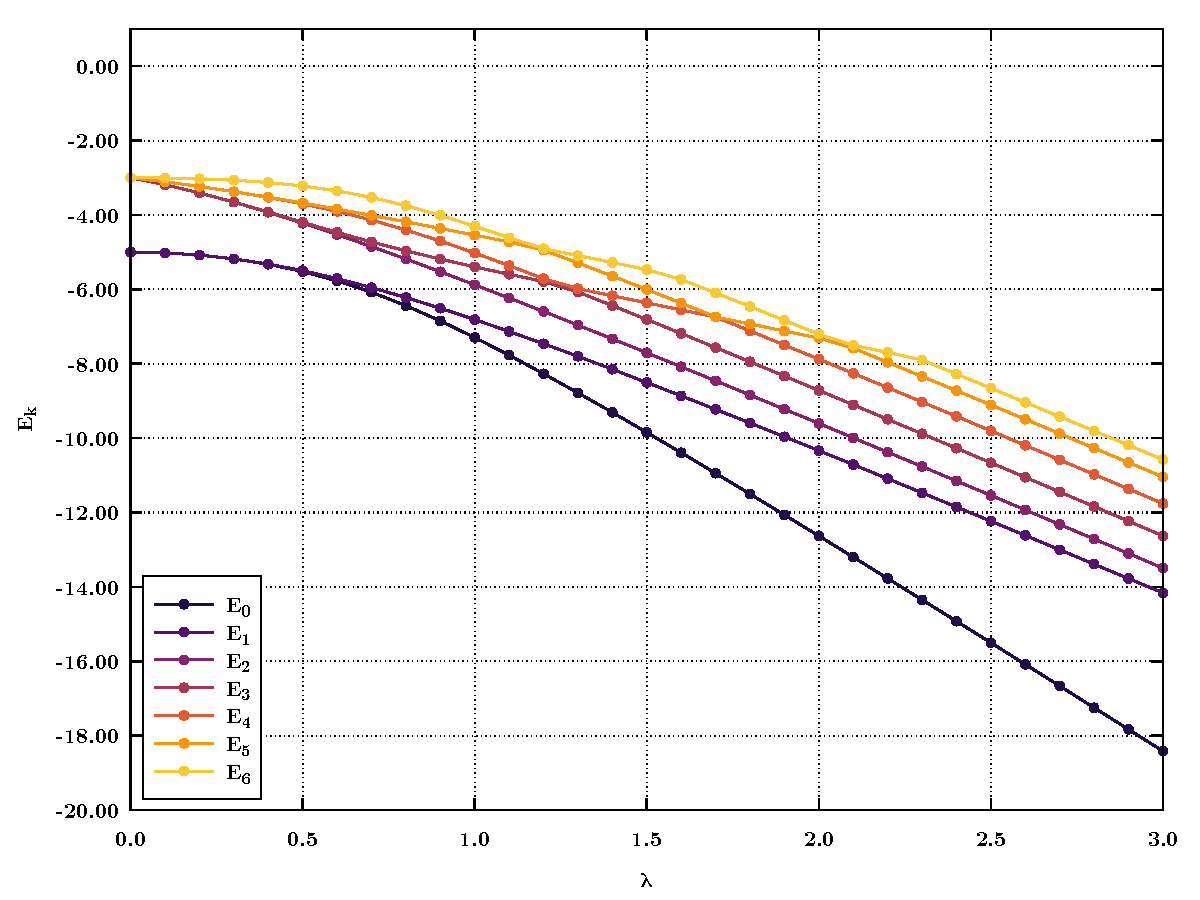
\includegraphics[width=\textwidth]{image/eig_6.pdf}  \label{fig:result(b)} }
\end{minipage} \\
\vfill
\begin{minipage}[c]{0.49\linewidth}
\subfloat[][8 particles]{ 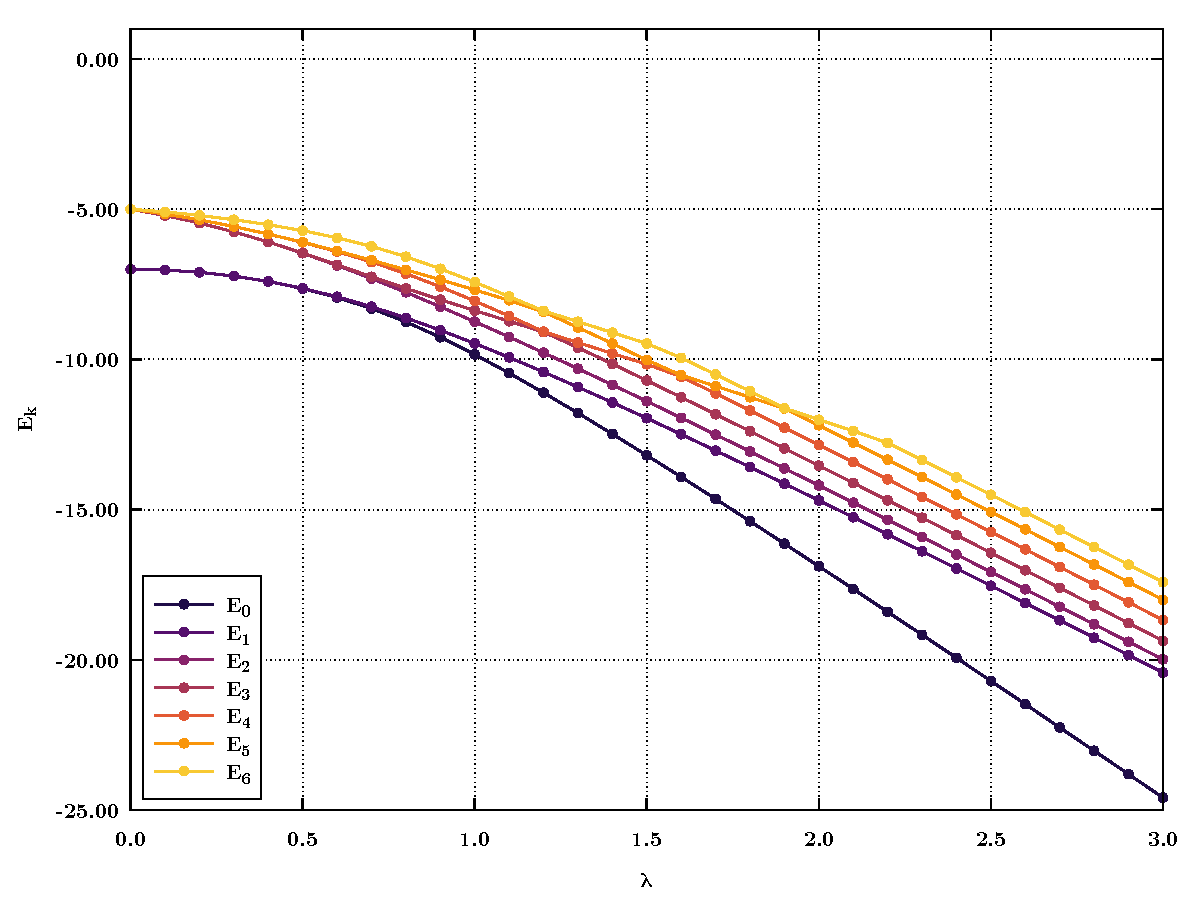
\includegraphics[width=\textwidth]{image/eig_8.pdf} \label{fig:result(c)} }
\end{minipage}
\begin{minipage}[]{0.49\linewidth}
\centering
\subfloat[][10 particles]{    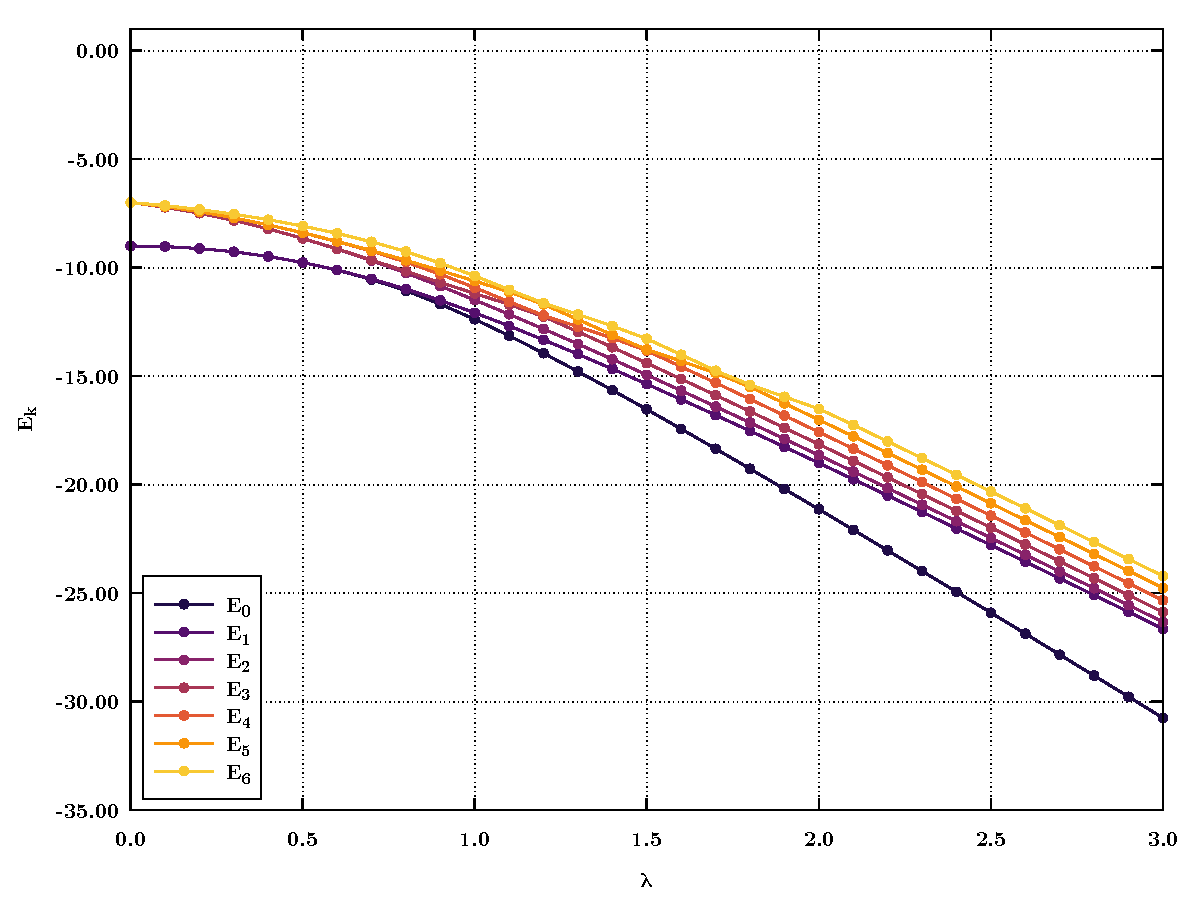
\includegraphics[width=\textwidth]{image/eig_10.pdf}  \label{fig:result(d)} }
\end{minipage}
\caption{\label{fig:results} Plots of the energy spectrum for the first 7 levels as a function of strength \( \lambda  \) for a different number of particles $N$. }
\end{figure}


\begin{figure}[H]
\centering
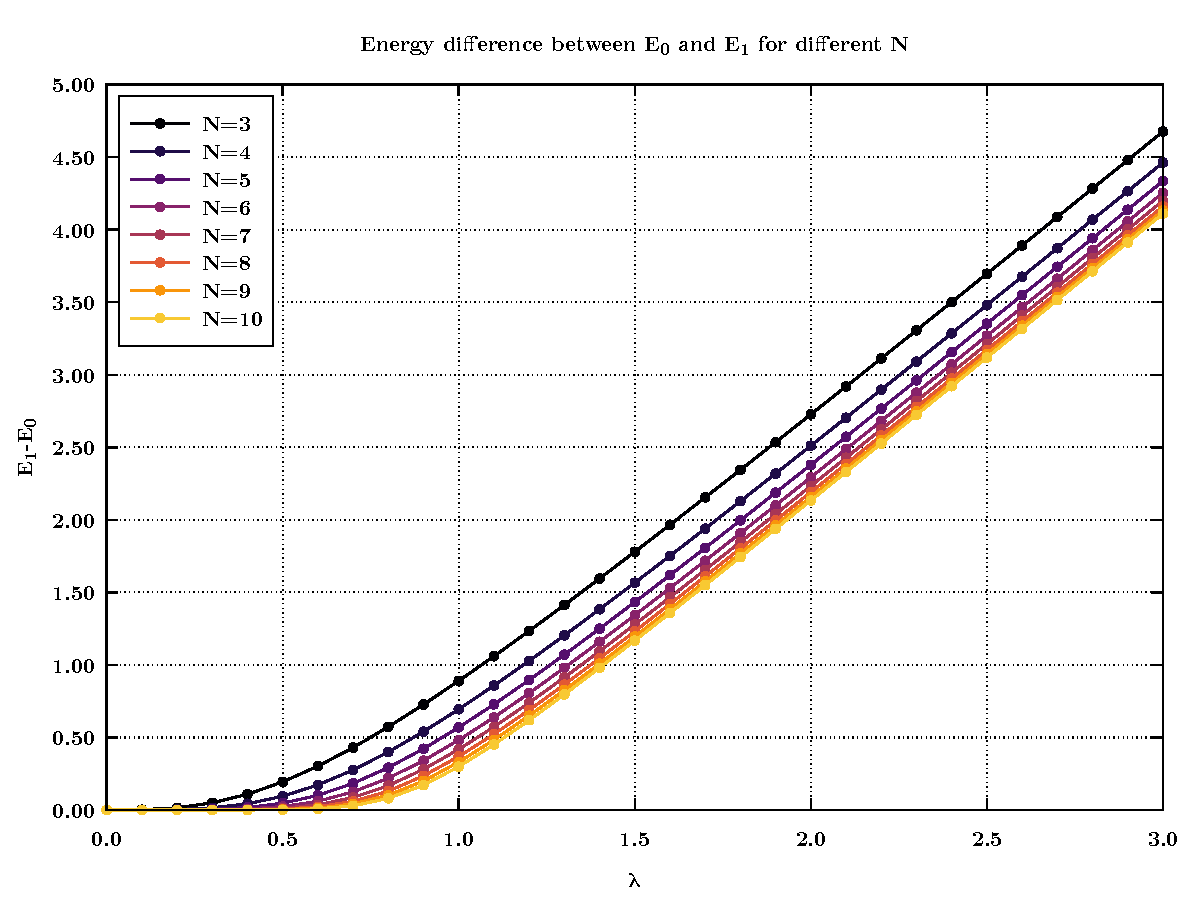
\includegraphics[width=0.7\textwidth]{image/diff.pdf}
\caption{\label{fig:diff} Difference between first excited state \( E_1 \) and ground state \( E_0 \) as a function of the interaction length \( \lambda  \) for different number of particles \( N \).}
\end{figure}

Now, let us focus on the case of $N=6$ particles. In Fig. \ref{fig:results_6}, we can see the energy spectrum for fixed values of the interaction strength.

As already mentioned, in Fig. \ref{fig:result_6(a)}, we notice that for \( \lambda =0 \) the ground state is two-fold degenerate. This corresponds to the case when all the spin are aligned down. In particular, the ground state energy is equal to $N-1=5$.
Furthermore, the first excited state turns out to be $2(N-1)=10$ degenerate.

Then, for \( \lambda =0.5 \) the degeneracy disappear as we can see in Fig. \ref{fig:result_6(b)}. However, in this case we note a trend of the energy states to be near in pairs. This trend completely fate away when \( \lambda = 1 \) and expecially for \( \lambda =3 \). Moreover, we note that by increasing the strength coefficient, the ground state level become more distant from all the other states.



\begin{figure}[h!]
\begin{minipage}[c]{0.49\linewidth}
\subfloat[][\( \lambda = 0 \)]{ 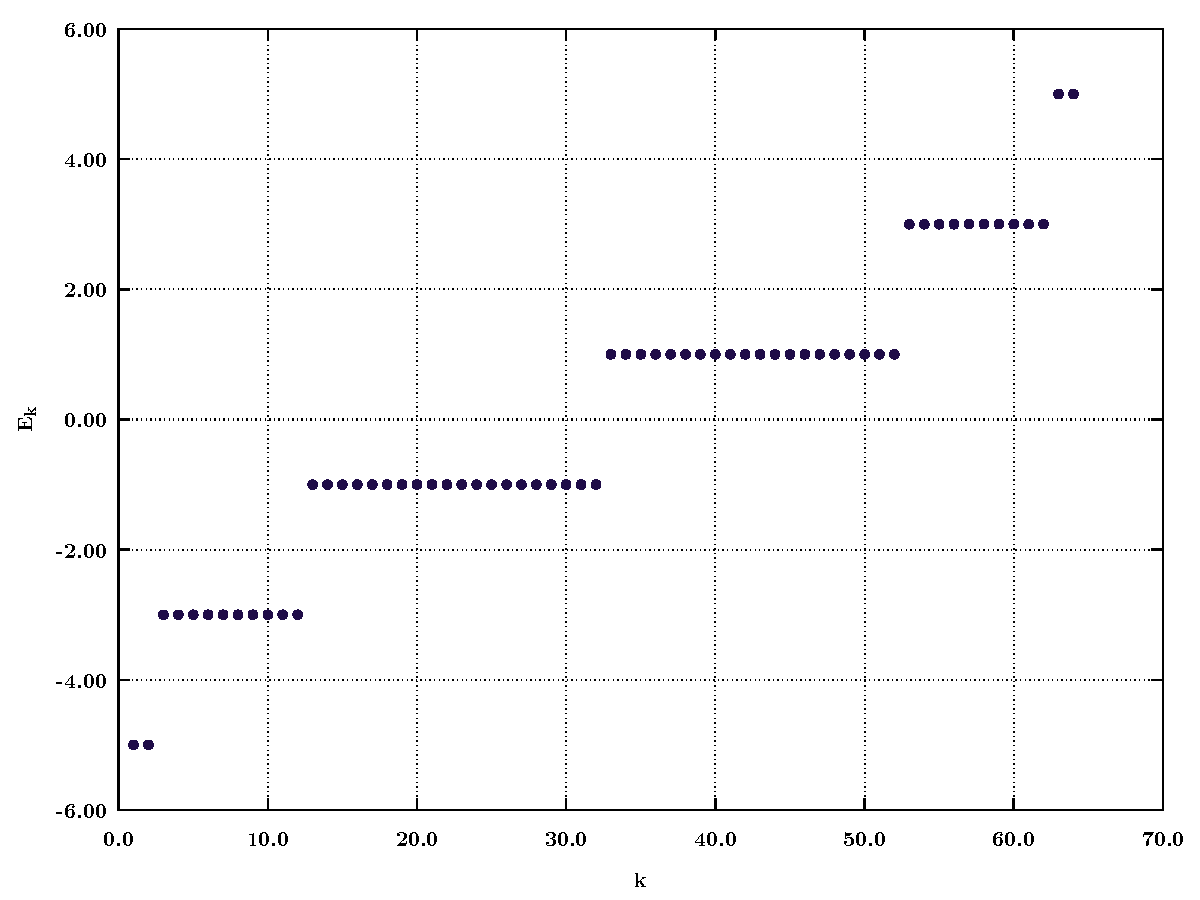
\includegraphics[width=\textwidth]{image/new_0_0_eig_6.pdf} \label{fig:result_6(a)} }
\end{minipage}
\begin{minipage}[]{0.49\linewidth}
\centering
\subfloat[][\( \lambda =0.5 \)]{    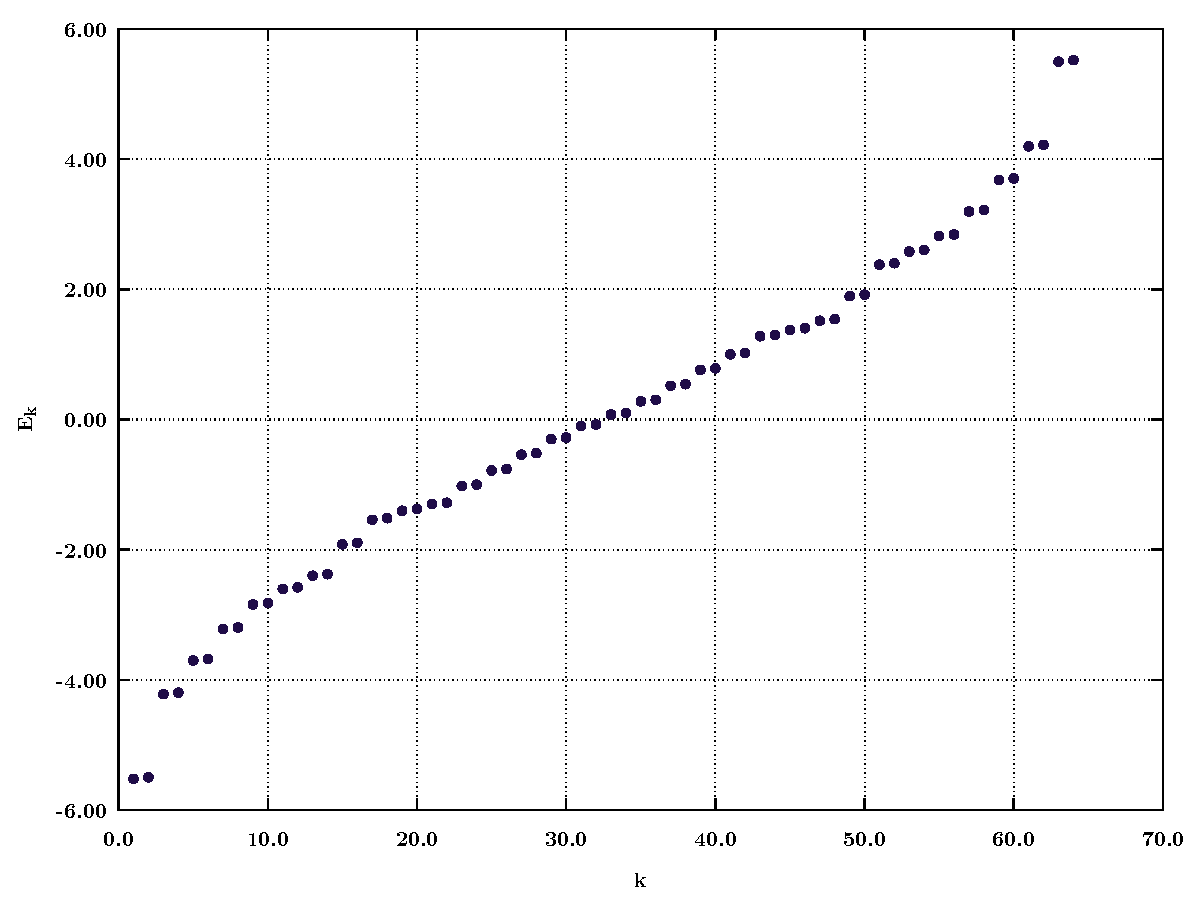
\includegraphics[width=\textwidth]{image/new_0_5_eig_6.pdf} \label{fig:result_6(b)} }
\end{minipage} \\
\vfill
\begin{minipage}[c]{0.49\linewidth}
\subfloat[][\( \lambda =1 \)]{ 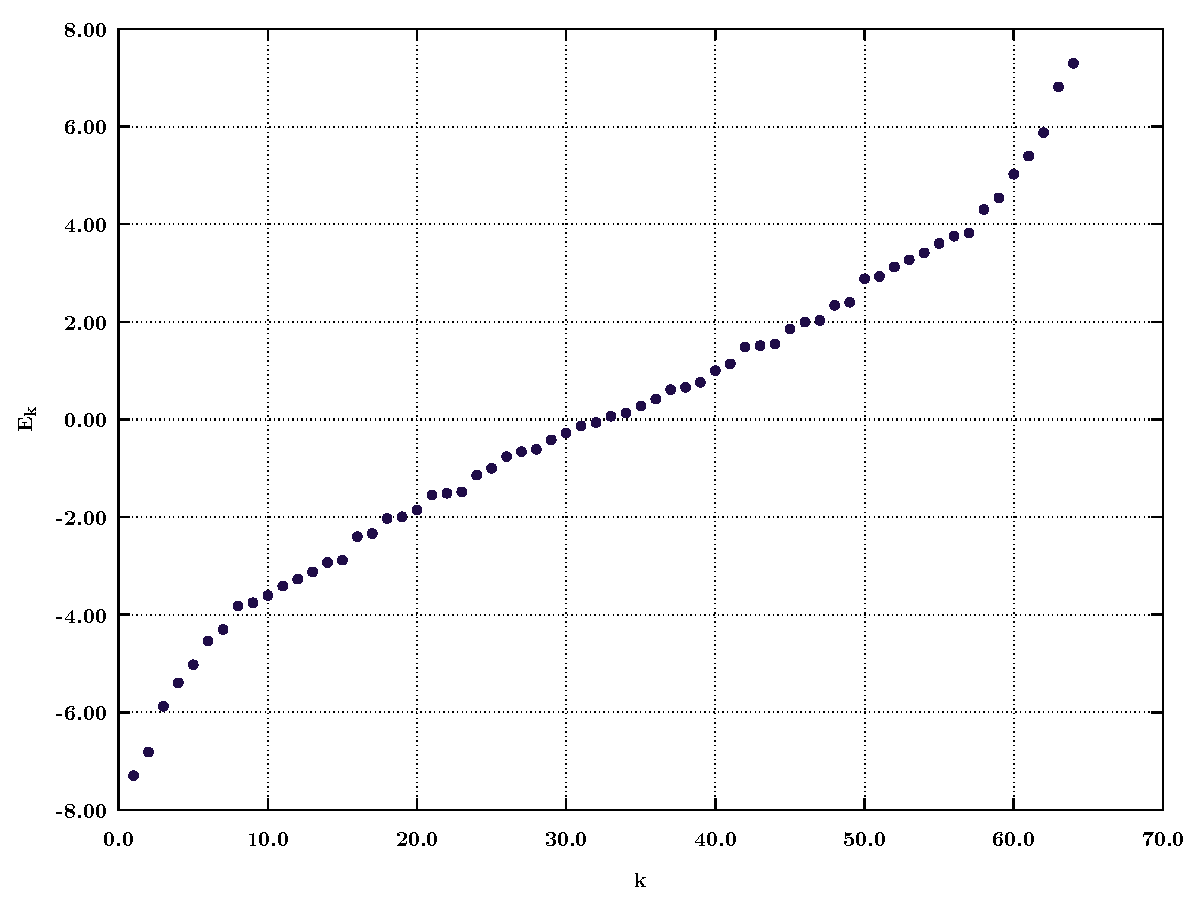
\includegraphics[width=\textwidth]{image/new_1_0_eig_6.pdf} \label{fig:result_6(c)} }
\end{minipage}
\begin{minipage}[]{0.49\linewidth}
\centering
\subfloat[][\( \lambda =3 \)]{    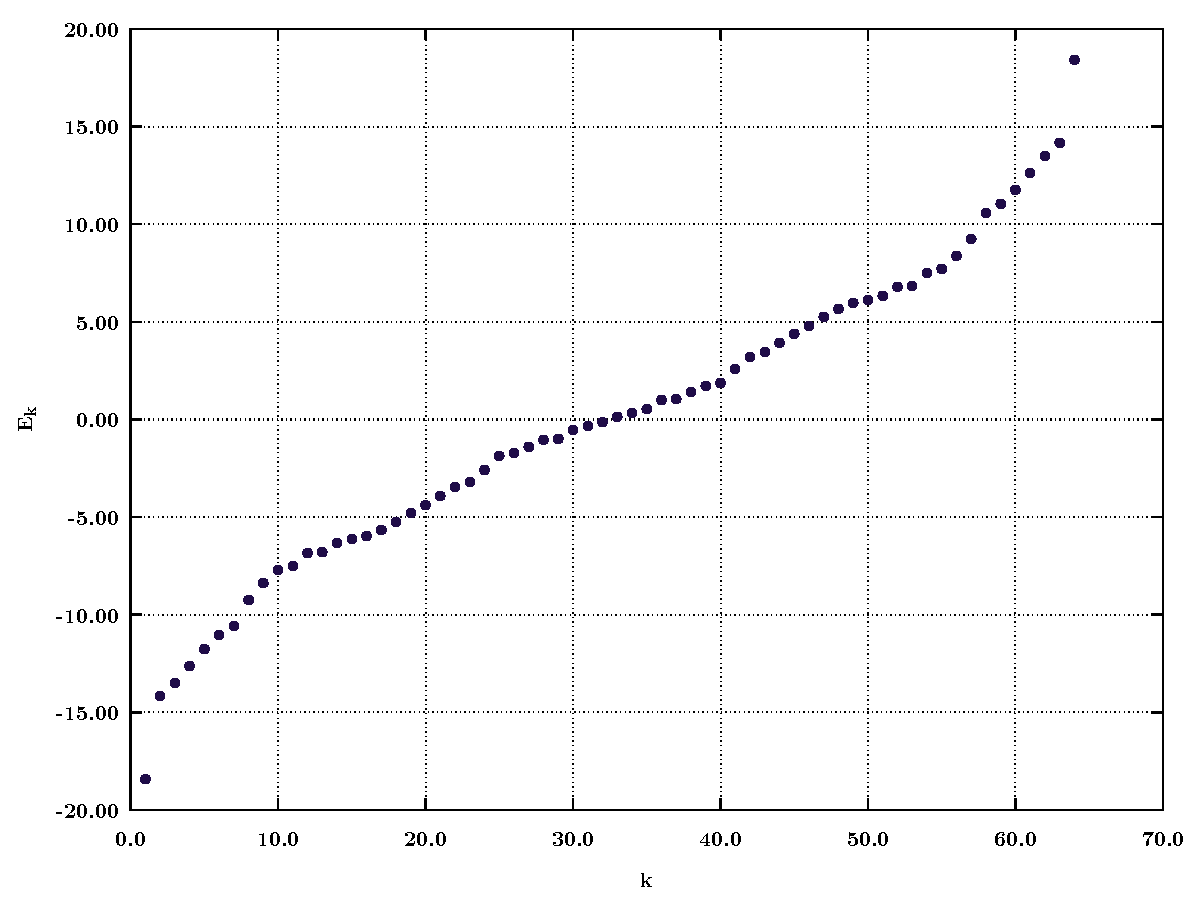
\includegraphics[width=\textwidth]{image/new_3_0_eig_6.pdf} \label{fig:result_6(d)} }
\end{minipage}
\caption{\label{fig:results_6} Plot of energy levels for an Ising model with 6 particles. }
\end{figure}

\section{Self-evaluation}
The code implemented works well and returns consistent results. In particular, we learn how to simulate a quantum Ising model and we study its spectrum for different values of the strength parameters \( \lambda  \).
In a further implementation of the code, it could be useful to optimize the function for the tensor product in order to be able to simulate systems with higher values of \( N \).





\end{document}
